\subsection*{\Large Общая характеристика работы}
\fontsize{14pt}{15pt}\selectfont


\textbf{Актуальность темы исследования.}
Популярность и стремительное развитие систем электронного обучения и платформ для массовых открытых онлайн-курсов MOOC (Massive Open Online Course) в последнее время привели к появлению огромного количества образовательных ресурсов, открытых, но практически никак не связанных между собой. Так крупнейший проект в области MOOC - Coursera насчитывает более 1000 онлайн-курсов, предоставленных более чем 100 университетами и организациями. Другими крупными MOOC порталами являются проекты EdX и Udacity, суммарная аудитория которых превышает 4 миллиона пользователей. В России проект <<ИНТУИТ>> позволяет пользователям бесплатно проходить обучение по более чем 800 онлайн-курсам, многие из которых касаются информационных технологий. Проект <<Лекториум>> занимается созданием и размещением открытых учебных курсов в формате видеолекций. Курсы проекта подготовлены ведущими ВУЗами и организациями России. Всего в проекте насчитывается более 4000 часов видеолекций. Отдельный вклад в увеличение количества образовательных ресурсов в сети Интернет внесли электронные библиотеки. Так Британская Библиотека предоставляет информацию о более чем 3,5 миллионах публикаций, книг и монографий в формате открытых данных с помощью проекта BNB (British National Bibliography). 

В области разработки систем обучения и автоматизации образовательных процессов возникает необходимость в сборе, агрегации, гармонизации и повторном использовании учебных материалов различных образовательных ресурсов в контексте одной системы электронного обучения. В настоящее время повторное использование учебных материалов сетевых образовательных ресурсов является одним из наиболее перспективных подходов для разработки систем электронного обучения. Разработка методик агрегации данных позволит создавать распределенные системы электронного обучения, использующие учебные материалы из различных образовательных ресурсов университетов, библиотек и организаций. Одним из методов реализации повторного использования учебных материалов в системах электронного обучения является применение семантических технологий. Технологии семантических сетей (Semantic Web) и связанных данных (Linked Data) позволяют системам обмениваться данными в сети с использованием онтологий и уникальных идентификаторов ресурсов URI (Uniform Resource Identifier). Автоматизация сбора, агрегации и гармонизации учебных материалов сетевых образовательных ресурсов в системе электронного обучения позволяет поддерживать содержание образовательного процесса в актуальном состоянии. При росте объемов учебных материалов и автоматизации наполнения системы электронного обучения возникает необходимость в контроле полноты, сбалансированности и целостности учебных курсов и программ. Семантические технологии позволяют формально описывать структуру и связи объектов образовательного процесса. На основе этих связей может быть разработана методика анализа полноты и сбалансированности учебного курса. 


Действия студентов в системе электронного обучения могут быть связаны с описанными формально объектами образовательного процесса. Разработка методики анализа деятельности пользователей на основе неявных связей с объектами образовательного процесса позволит преподавателям и авторам курсов получить отклик от студентов. На основе анализа полноты, целостности курсов, а так же на основе откликов студентов, авторы курсов и преподаватели могут вносить коррективы в образовательный процесс с целью повышения качества обучения. Аналитическая информация деятельности студентов в системе позволит студентам производить мониторинг процесса обучения.     

\textbf{Целью диссертационной работы} является исследование и разработка методов агрегирования и анализа образовательных данных в системе электронного обучения с использованием семантических технологий.

Для достижения поставленной цели необходимо было решить следующие \textbf{задачи}:
\begin{enumerate}
 \item Разработать онтологические модели для описания учебных материалов, тестов, предметных областей учебных дисциплин, результатов и процесса обучения студентов, показателей оценки знаний и рейтинга студентов;
 \item Разработать методику автоматического агрегирования образовательных данных в системе электронного обучения с использованием методов естественной обработки языка, логического вывода, технологий Semantic Web и Linked Data;
 \item Разработать метод анализа полноты и сбалансированности образовательных материалов, основанный на семантических связях в онтологических моделях;
  \item Разработать алгоритм автоматизированной оценки результатов обучения и построения рейтингов студентов системы электронного обучения с использованием статистических методов и семантических технологий;
  \item Создать программные модули для системы электронного обучения на основе разработанных методов;
  \item Внедрить созданные программные модули в систему электронного обучения и провести экспериментальные исследования с участием студентов.  
 \end{enumerate}

\textbf{Объектом исследования} является структура и логические отношения между объектами образовательного процесса, предметных областей учебных дисциплин и образовательных ресурсов.  

\textbf{Предметом исследования} является алгоритмическое обеспечение, предназначенное для автоматизации процессов наполнения системы электронного обучения учебными материалами, процессов анализа полноты и сбалансированности учебных материалов и знаний студентов. 

\textbf{Новые научные результаты.}
\begin{enumerate}
 \item Онтологическая модель, описывающая образовательный процесс, учебные материалы, предметные области, действия студентов и отношения между данными объектами. 
 \item Метод оценки полноты и сбалансированности учебного курса на основе анализа неявных семантических связей.
\end{enumerate}

\textbf{Основные положения, выносимые на защиту.}
\begin{enumerate}
 \item Модульная онтология, описывающая структуру образовательного процесса, структуру предметной области учебной дисциплины, структуру тестов, действия и результаты студентов в системе электронного обучения.
 \item Методика наполнения образовательной онтологии и агрегации учебных материалов в системе электронного обучения;
 \item Метод анализа полноты и сбалансированности электронного курса на основе разработанной онтологии;
 \item Алгоритм анализа знаний и рейтинга студентов системы электронного обучения.
 \end{enumerate}


\textbf{Практическая значимость.}
\begin{enumerate}
 \item Разработанная модульная онтология опубликована в сети с зарегистрированными идентификаторами PURLs (Persistent Uniform Resource Locators) и может быть использована для разработки систем электронного обучения.
 \item Программная реализация системы электронного обучения, использующая разработанные модели и алгоритмы, была внедрена на открытой площадке на кафедре проектирования и безопасности компьютерных систем Университета ИТМО (ecole.ifmo.ru). 
 \item Онтологии, созданные на основе разработанных моделей и алгоритмов, используются на практике в онлайн курсах <<Интеллектуальные системы>>, <<Физика>>, <<Теория графов>> и <<Аналитическая геометрия и линейная алгебра>>.
 \end{enumerate}
 
 
%\textbf{Достоверность} изложенных в работе результатов обеспечивается ...


\textbf{Апробация работы.}
Основные результаты диссертационной работы докладывались и обсуждались на следующих конференциях:
International Conference on Knowledge Engineering and Semantic Web (Россия, Санкт-Петербург, 2013),
11th Extended Semantic Web Conference (Греция, Аниссарас, 2014), International Conference on Knowledge Engineering and Semantic Web (Россия, Казань, 2013), The 13th International Semantic Web Conference (Италия, Рива-дель-Гарда, 2014), 16th Conference of Open
Innovations Association FRUCT (Финляндия, Оулу, 2014), 24th World Wide Web Conference (Италия, Флоренция, 2015).

\textbf{Публикации.} Основные результаты по теме диссертации изложены в 8 печатных изданиях, 8 из которых изданы в журналах, рекомендованных ВАК.

\textbf{Объем и структура работы.} Диссертация состоит из введения, четырех глав, заключения и приложения. Полный объем диссертации \textbf{124} страниц текста с \textbf{48} рисунками и \textbf{5} таблицами. Список литературы содержит \textbf{120} наименований.

%\newpage
\subsection*{\Large Содержание работы}
Во \textbf{введении} обосновывается актуальность исследований, проводимых в рамках данной диссертационной работы, приводится обзор научной литературы по изучаемой проблеме, формулируется цель, ставятся задачи работы, сформулированы научная новизна и практическая значимость представляемой работы.

\textbf{Первая глава} посвящена обзору и анализу семантических технологий для автоматизации процессов в системах электронного обучения. В главе описывается основной функционал и особенности систем электронного обучения и приводится краткая история этапов их развития. На основе анализа отечественных и зарубежных систем электронного обучения и образовательных ресурсов были сформированы имеющиеся проблемы в области дистанционного образования. В данный момент в системах электронного обучения отсутствуют механизмы автоматической агрегации и анализа образовательных данных с использованием открытых образовательных ресурсов. Отсутствие семантического содержания в данных систем электронного обучения значительно снижает возможности проведения анализа данных на основе косвенно выводимых фактов.

В главе описываются теоретические основы онтологий, семантических технологий и концепции Linked Data. В главе раскрываются понятия онтологии, экспертной системы, базы знаний и семантической сети. Также приводится краткое описание основных стандартов, протоколов и форматов хранения данных в семантических технологиях.

Онтология - термин, заимствованный из философии, который обозначает науку, описывающую формы бытия и то, как они относятся между собой. Иными словами онтология - это явное описание концептуализации. Основными структурными элементами языка онтологий являются понятия класса, индивида и свойства. Онтологии в общем виде определяемые как совместно используемые формальные концептуализации конкретных предметных областей, дают общее представление о темах, информацией по которым могут обмениваться люди и приложения. Назначением экспертных систем является автоматизация деятельности человека. Ядром экспертной системы является база знаний. База знаний является совокупностью  знаний предметной области, записанной на машинный носитель в форме, понятной эксперту и пользователю.

Семантическая сеть является  методом представления знаний и позволяет описывать объекты, явления и понятия предметной области с помощью теории графов. Характерной особенностью семантических сетей является обязательное наличие трех типов отношений: класс, свойство и экземпляр класса. Главной целью семантической сети является хранение мировой информации в виде пригодном для машинной обработки. Основной моделью описания данных в семантической сети является модель RDF(Resource Description Framework).  RDF представляет утверждения о ресурсах в виде триплетов. Триплет состоит из субъекта, предиката и объекта. Субъект, объект и предикат определяются с помощью URI. Существует множество форматов представления и хранения данных RDF таких, как XML и N-Triples. Для описания синтаксиса классов объектов используется язык описания онтологий OWL (Ontology Web Language). OWL позволяет явно описывать свойства и классы: наследование классов, характеристики свойств, мощность связей и эквивалентность. Для произведения запросов к семантическим данным используется протокол SPARQL (SPARQL Protocol and RDF Query Language). SPARQL позволяет получать доступ к данным в формате RDF через стандартизированный интерфейс и язык запросов. Организация SPARQL точки доступа к данным позволяет пользователям и приложениям получать данные из базы знаний.

Концепция Linked Data предполагает использование Web-технологий HTTP, RDF, и URI для публикации данных в сети и объединения данных из разных источников. Данная концепция позволяет данным из одного источника ссылаться на данные другого источника. В соответствии с концепцией все элементы определяются по средствам URI и переход по URI ведет к получению большего количества данных об элементе. Наборы данных должны включать в себя ссылки на другие источники для возможности проведения дальнейшей навигации по данным вне одного ресурса. В данный момент опубликованные наборы связанных данных охватывают информацию о географических локациях, людях, компаниях, книгах, научных публикациях, фильмах, музыке, телевидении и радио, лекарствах, генах и о многом другом.

В главе производится анализ исследовательских работ по сформированным в начале главы проблемам. В главе описываются последние исследования в области применения семантических технологий в системах электронного обучения. Последние исследования показывают, что использование технологий Semantic Web и Linked Data позволяет автоматизировать наполнение системы определенными данными из открытых источников. Семантические технологии в системе электронного обучения позволяют решить такие проблемы, как наполнение и поддержка актуальности учебных материалов в системе, оценка полноты и сбалансированности учебного курса, автоматизация проверки знаний студентов.

В конце главы на основе проведенного анализа применения семантических технологий в системах электронного обучения сформирован подход к автоматизированной агрегации и анализу данных в системах электронного обучения с использованием семантических технологий. 

\textbf{Вторая глава} посвящена разработке онтологической модели для описания структуры образовательного процесса, структуры предметной области учебной дисциплины, структуры тестов, действий и результатов студентов в системе электронного обучения.

В результате анализа систем электронного обучения была сформирована общая модель данных в системе. Модель делится на три основных уровня: уровень предметных областей, уровень учебных материалов, уровень деятельности пользователей в системе. Уровни модели связаны друг с другом для обеспечения взаимодействия различных ресурсов системы. Уровень предметных областей является основой модели данных и содержит информацию о предметных областях учебных дисциплин. Сбор данных для этого уровня производится из открытых, опубликованных баз знаний, таксономий и наборов данных. Уровень учебных материалов содержит информацию необходимую для проведения учебного процесса. На данном уровне хранятся данные по образовательным программам, курсам, тестам и медиа-ресурсам. На данном уровне хранится информация о предметных областях и их концептах. Сбор данных для этого уровня производится из хранилищ университетов, открытых электронных библиотек и медиа-ресурсов. Связывание учебных материалов с концептами и предметными областями производится в полуавтоматическом режиме с использованием алгоритмов обработки естественного языка. Уровень деятельности пользователей в системе содержит результаты обучения студентов и  статистические данные по активности пользователей. Статистика ведется в системе управления обучением LMS (Learning Management System). При ведении статистики используется информация из социальных сетей. Связывание статистики и результатов обучения с учебными материалами происходит в автоматическом режиме алгоритмами LMS. Общая модель данных системы электронного обучения представлена на рисунке \ref{fig:OverallModel}. 

\begin{figure}[ht] 
  \center
  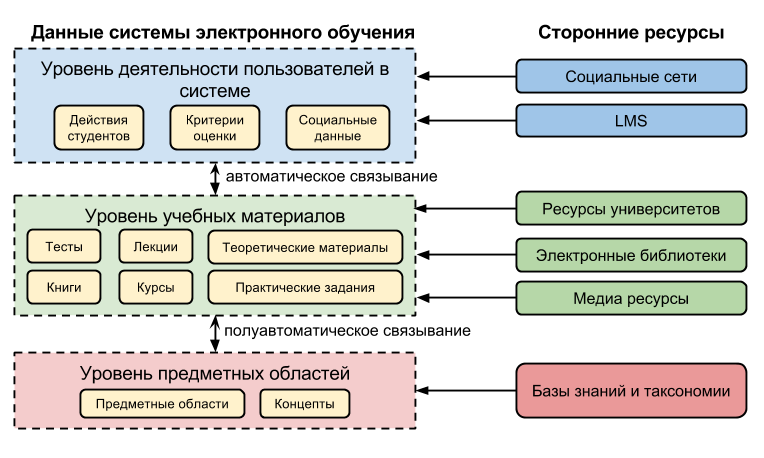
\includegraphics[scale=0.5]{OverallModel}
  \caption{Общая модель данных системы электронного обучения} 
  \label{fig:OverallModel}
\end{figure}

На основе описанной общей модели данных системы была разработана модульная онтология. Модульная онтология состоит из следующих модулей:


\begin{itemize}
\item Модуль учебных материалов - онтология, которая описывает отношения между курсами, модулями, лекциями, тестами, практиками и концептами предметной области;
\item Модуль тестов - онтология, которая описывает содержание тестов, вопросы, ответы, варианты тестов;
\item Модуль действий и результатов студента в системе обучения - онтология, которая позволяет хранить статистику по действиям студентов в системе и результаты обучения студентов, включая правильные и неправильные ответы на тесты, прохождения лекций и результаты экзаменов.
\item Модуль оценки знаний студентов - онтология, которая позволяет хранить вычисленные автоматически оценки знаний студентов по определенным концептам и предметным областям.
\end{itemize}

Модуль учебных материалов основан на онтологиях верхнего уровня, рекомендованных к использованию при описании учебных материалов. При разработке данного модуля использовались онтологии AIISO (The Academic Institution Internal Structure Ontology), BIBO (The Bibliographic Ontology) и MA-ONT (The Ontology for Media Resources). Модуль учебных материалов является связующим звеном для всех модулей разработанной онтологии. Одной из главных особенностей разработанной онтологии является возможность произведения прямого и косвенного междисциплинарного связывания объектов электронных курсов. 




\textbf{Третья глава} посвящена исследованию методов автоматического агрегирования образовательных данных и разработке методов и подходов к автоматизированной оценке полноты и сбалансированности учебных курсов и результатов обучения студентов.  

В главе описывается разработанная методика по агрегации и гармонизации учебных материалов в системе электронного обучения. Технологии Semantic Web и Linked Data позволяют использовать онтологии для хранения, сбора и распространения данных. Одним из преимуществ данных технологий является повторное использование данных. В Интернете существует множество открытых источников с данными, при описании которых были использованы онтологии верхнего уровня. Данные источники могут быть использованы для наполнения системы электронного обучения. Для сбора и интеграции данных в системе электронного обучения предлагается использовать провайдеры данных. Провайдеры данных -- это программные модули, поддерживающие автоматическое обновление связанных данных из открытых источников, используя определенные алгоритмы. Провайдеры позволяют преобразовывать структурированные данных различных форматов в формат RDF. Каждый провайдер обладает своим контекстом для дальнейшего управления собранными данными. В результате исследования был сформирован следующий набор методов агрегации данных:

\begin{itemize}
\item интеграция связанных данных из открытых источников в формате RDF на примере связывания учебных курсов с данными электронной библиотеки BNB;
\item интеграция и преобразование структурированных данных в форматах XML и JSON в формат RDF с использованием отображения на примере адаптации тестов Университета ИТМО;
\item интеграция результатов SPARQL запросов к открытым точкам доступа на примере сбора определений для концептов предметных области из электронной энциклопедии DBpedia;
\item интеграция результатов REST запросов с использованием отображения на примере связывания учебных курсов с данными портала учебных изданий Университета ИТМО;
\item применение методов обработки естественного языка для создания дополнительных связей между объектами на примере связывания концептов с заданиями учебных тестов.
\end{itemize}

Особое внимание в главе уделяется применению методов обработки естественного языка для гармонизации объектов в онтологии. Для наполнения онтологий системы можно использовать не только данные внешних источников, но и данные самой системы. Данные, хранящиеся в онтологии системы, позволяют создавать новые связи на основе предопределенных правил. Используя методы обработки естественного языка, можно извлекать семантические связи из текстовой информации объекта онтологии. В исследовании данные методы использовались для выявления связей между концептами и заданиями теста. В тексте вопроса задания и его ответов производился поиск концептов. Найденные концепты связывались с заданиями теста. Данные связи обозначали использование концепта предметной области в задании учебного теста и позволяли формально описать содержание задания. 

Для реализации алгоритма связывания заданий тестов и концептов предметной области был разработан провайдер данных. Провайдер принимает на вход ссылку на объект курса и производит создание ссылок между заданиями и концептами. Для извлечения концептов была использована лингвистическая платформа NooJ. Общий алгоритм работы провайдера данных представлен на рисунке \ref{fig:NLPAlgo}.

\begin{figure}[ht] 
  \center
  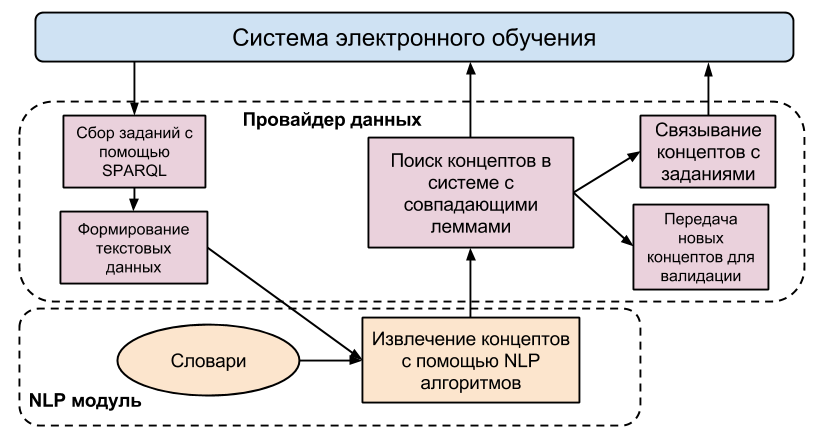
\includegraphics[scale=0.45]{NLPAlgo}
  \caption{Алгоритм работы провайдера данных для извлечения концептов с использованием методов обработки естественного языка} 
  \label{fig:NLPAlgo}
\end{figure}

Концепты-кандидаты, для которых не были найдены соответствующие концепты системы, могут быть записаны в онтологию, как новые концепты системы. Перед записью в онтологию провайдер производит проверку концепта-кандидата на соответствие концепту предметной области. Для проверки используются запросы к базе знаний DBpedia. Для включения нового концепта в систему необходима верификация преподавателя или администратора системы. 

Далее в главе описывается разработка метода анализа полноты и сбалансированности  учебного курса. Метод основан на анализе косвенных связей в онтологии системы. Аналитика формируется из статистических данных, полученных с помощью SPARQL запросов. 

Одним из примеров использования метода является анализ покрытия лекций курса тестами и заданиями. В онтологии системы лекции и тесты связаны с определенным модулем курса. В результате работы алгоритмов по наполнению онтологий лекции и задания тестов могут быть связаны с определенными концептами. Таким образом, происходит косвенное связывание лекций и тестов через концепты. Если концепт лекции использован в задании теста, он считается покрытым в данном модуле учебного курса.

Другим подходом к анализу учебных материалов является выявление проблемных концептов предметной области в модуле учебного курса. Проблемными концептами являются концепты, при изучении которых у студентов возникают наибольшие затруднения. Статистика по результатам прохождения студентами тестов, правильные и неправильные ответы на задания, связанные с определенными концептами, позволяют рассчитать общий рейтинг знания студентами определенного концепта. Используя данный рейтинг, преподаватель может получить список концептов курса, которых студенты знают хуже всего. Это позволит преподавателю вносить коррективы в учебные материалы и учебный процесс. В текущей реализации метода используется упрощенная формула расчета рейтинга проблемного концепта. Рейтинг проблемного концепта рассчитывается делением количества неправильных ответов на количество правильных ответов на задания, связанные с данным концептом. Данная формула может быть усовершенствована с помощью включения дополнительных параметров. Рейтинг проблемных концептов для модуля составляется с помощью следующего  SPARQL-запроса:

\begin{verbatim}
    SELECT ?term 
        (count(?correct_answer) AS ?correct_answer_count)
        (count(?answer) AS ?answer_count)
        ((2*?correct_answer_count - ?answer_count) 
            AS ?rank) 
    WHERE{
        ?module learningRu:hasTest ?test  . 
        ?test ifmotest:hasGroupOfTasks 
            ?group_of_tasks .        
        ?group_of_tasks ifmotest:hasTask ?task .      
        ?test_element lres:hasTask ?task .
        ?test_element lres:hasAnswer ?answer .
        ?task learningRu:hasTerm ?term .       
        OPTIONAL { 
            ?task ifmotest:hasCorrectAnswer 
                ?correct_answer
            filter( ?correct_answer = ?answer)
        }         
    }
    GROUP BY ?term 
    ORDER BY ASC(?rank)
\end{verbatim}


Аналитка полноты и сбалансированности учебного курса состоит из следующей статистической информации:
\begin{itemize}
\item количество покрытых и непокрытых концептов в модуле учебного курса;
\item общий процент покрытия модуля тестами на основе отношения покрытых концептов к общему количеству концептов;
\item облако тегов концептов модуля, демонстрирующее полноту и степень покрытия каждого концепта;
\item список непокрытых концептов модуля, которые были использованы в лекциях, но не были использованы в заданиях тестов;
\item список проблемных концептов с рейтингами в модуле учебного курса;
\item диаграмма отношений между пятью самыми проблемными концептами модуля учебного курса.
\end{itemize}


В конце главы описывается алгоритм автоматизированной оценки результатов обучения и построения рейтингов студентов системы электронного обучения с использованием статистических методов и семантических технологий. Данный алгоритм позволяет студентам получать информацию о своих знаниях по концептам и предметным областям учебных дисциплин в режиме реального времени. Такая информация может использоваться студентами для выявления пробелов в знаниях и при повторении пройденных учебных материалов. Полученная информация о знаниях и результатах позволит формировать рекомендации для студентов по образовательным программам, исследовательским проектам и лабораториям. Преподаватели смогут использовать информацию о знаниях и результатах студентов во время подготовки к проведению учебного курса и лекций у определенной группы студентов.

Алгоритм основан на семантическом анализе действий студентов в системе электронного обучения в проекции образовательного процесса и учебных материалов. Алгоритм позволяет производить автоматизированную оценку знаний студентом определенной предметной области учебной дисциплины. Оценка знания студентом предметной области основывается на расчете рейтинга знания студентом соответствующей предметной области. Рейтинг знания студентом предметной области зависит от рейтингов знания студентом концептов, входящих в данную предметную область. Расчет рейтинга знания студентом концепта зависит от показателей оценки действий студента в системе. Набор показателей может варьироваться в зависимости от возможных действий студента в системе, структуры онтологии и необходимой точности вычислений. В предложенном подходе используется показатель знакомства студента с концептом и показатель проверки знания студентом концепта с помощью тестов. Расчет рейтинга знания студентом предметной области производится с учетом значимости (важности) концептов в образовательном процессе.

Рейтинг знания студентом концепта, как и рейтинг знания студентом предметной области, варьируется от 0 до 1. Показатель знакомства студента с концептом является бинарным показателем и обозначает факт изучения студентом концепта с использованием теоретического материала. В разработанном подходе изучением концепта является завершение студентом лекции, связанной с данным концептом в системе электронного обучения. Изучить концепт предметной области студент может только один раз. В разработанном подходе данный показатель составляет 15\% от общего рейтинга знания студентом концепта.

Показатель проверки знания студентом концепта с помощью тестов основан на статистическом анализе правильных и неправильных ответов студента на задания учебных курсов, которые связаны с данным концептом. В разработанном подходе данный показатель составляет 85\% от общего рейтинга знания студентом концепта. Показатель рассчитывается как нижняя граница доверительного интервала Вильсона для параметра Бернулли по количеству правильных и неправильных ответов студента на задания, используя формулу:

$$
    R_t = \frac{p+\frac{1}{2n}z_{1-\alpha/2}^2 \pm z_{1-\alpha/2}\sqrt{\frac{p(1-p)}{n}+\frac{z_{1-\alpha/2}^2}{4n^2}}{} }{1+\frac{1}{n}z_{1-\alpha/2}^2},
$$

где \(z_{1-\alpha/2}\) - квантиль от \(1-\alpha/2\) стандартного нормального распределения, \(p\) - доля правильных ответов от общего количества ответов, \(n\) - общее количество ответов. 

Сумма двух полученных показателей для концепта в соответствии с их долями является общим рейтингом знания студентом концепта. Предметные области и концепты в соответствии с разработанной моделью не зависят от учебных материалов и могут повторно использоваться во множестве учебных курсов. Связи между концептами, описывающие необходимость одного концепта для изучения другого, позволяют рассчитать значимость концепта в образовательном процессе. Чем больше концептов, для изучения которых необходим определенный концепт, тем выше значимость данного концепта. При расчете учитывается количество концептов на разных уровнях зависимости. Уровнем зависимости является глубина косвенной зависимости одного концепта от другого через набор концептов. Например, на втором уровне зависимости находятся концепты, зависимые от концептов, зависимых от рассматриваемого концепта предметной области. Значимость концепта рассчитывается с использованием трех уровней зависимости по формуле: 

$$
    W_t = \frac{1}{e}+\sum_{k=1}^{3}\frac{n_{tk}}{e^k}, 
$$

где \(n_{tk}\) - количество концептов, связанных с данным концептом на каждом уровне зависимости, \(k\) - номер зависимого уровня, \( \frac{1}{e} \) - константное значение концепта. 

Итоговый рейтинг знания студентом предметной области учебной дисциплины рассчитывается как сумма рейтингов знания студентом концептов, входящих в предметную область. При расчете необходимо учитывать относительную значимость концепта в предметной области. Для этого необходимо рассчитать суммарную значимость предметной области, используя формулу:

$$  
    W_f = \sum_{i=1}^{n}W_{ti},
$$

где \(W_{ti}\) - значимость концепта предметной области, \(n\) - количество концептов в предметной области.

Относительная значимость концепта в предметной области рассчитывается по формуле:

$$
    D_t = \frac{W_t}{W_f},
$$

где \(W_t\) - значимость концепта, \(W_f\) - значимость предметной области.

Рейтинг знания студентом предметной области является суммой рейтингов знания студентом концептов в соответствии с их относительными значимостями:

$$
    R_f = \sum_{i=1}^{n} R_{ti}D_{ti},
$$
где \(R_{ti}\) - рейтинг знания студентом концепта, \(D_{ti}\) - относительная значимость концепта в предметной области.

Представленный алгоритм позволяет производить автоматизированную оценку знания студентами предметных областей. Поддержка набора показателей позволяет системе варьировать алгоритмы расчета оценки, добавляя, изменяя и удаляя необходимые показатели. Помимо оценки предметных областей данный подход можно применять к любым объектам образовательного процесса, напрямую или косвенно связанным с концептами. Алгоритм позволяет производить оценку знаний студентами учебных курсов и специальностей.  

В \textbf{четвертой главе} приведено описание архитектуры и особенности реализации программных модулей для системы электронного обучения. Также в главе описаны основные результаты исследований по разработанным методикам.

\begin{figure}[ht] 
  \center
  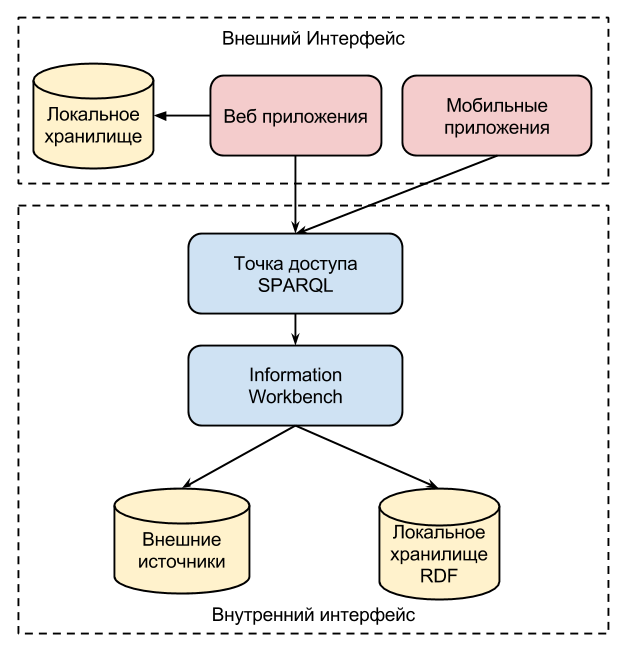
\includegraphics[scale=0.40]{OverallArch}
  \caption{Общая архитектура системы электронного обучения ECOLE} 
  \label{fig:OverallArch}
\end{figure}


На основе разработанных моделей и методик были реализованы программные модули, которые в своей комбинации формируют ядро системы электронного обучения ECOLE (Enhanced Course Ontology for Linked Education). Сервер системы ECOLE реализован на языке Java и основан на платформе Information Workbench. Платформа Information Workbench предоставляет функционал для работы с открытыми связанными данными. Редактирование и управление RDF данными системы реализовано с использованием платформы OpenRDF Sesame. Сервер системы ECOLE предоставляет открытую точку доступа для SPARQL запросов. 

Внешним интерфейсом системы электронного обучения ECOLE является LMS. LMS обладает локальным хранилищем и производит управление пользовательскими данными, настройками и результатами обучения студентов. В LMS реализованы модули для отображения видеолекций, слайдов, тестов и практических заданий. Внешний интерфейс получает с сервера данные по учебным материалам и отношения между объектами курса с помощью запросов к открытой точке доступа SPARQL. Персональные данные пользователей и настройки LMS хранятся в локальной памяти внешнего интерфейса. С помощью алгоритмов LMS производится сбор статистических данных по действиям студентов в системе и запись их в онтологии на сервере системы. LMS реализована на языке Python с использованием Django Web Framework. Общая архитектура системы электронного обучения ECOLE представлена на рисунке \ref{fig:OverallArch}.



После прохождения теста система предоставляет студенту информацию о количестве и доле правильных ответов на задания теста и список концептов для повторения. На основе разработанных методов система рассчитывает рейтинг знания студентом  концептов и областей (Рисунок \ref{fig:screen2}).

\begin{figure}[ht] 
  \center
  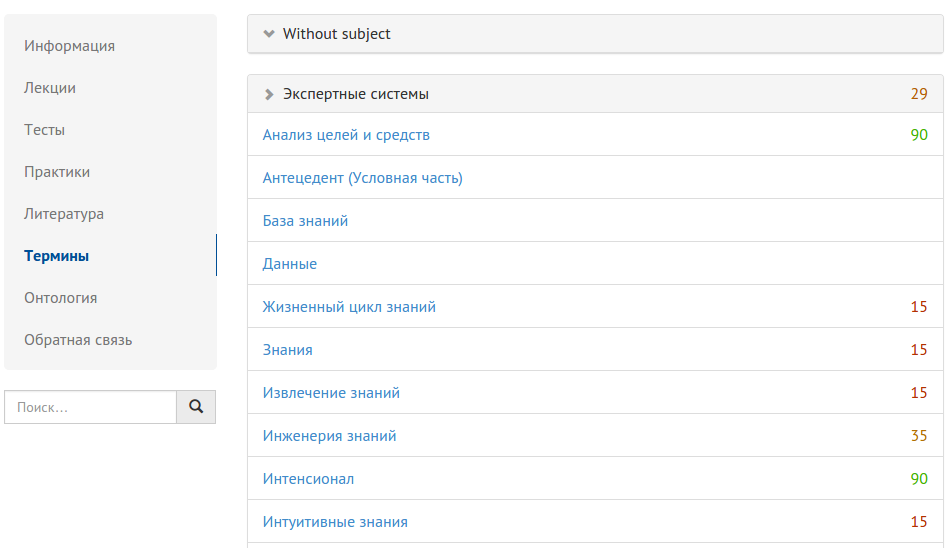
\includegraphics[scale=0.40]{screen2}
  \caption {Интерфейс списка предметных областей и концептов с рейтингами знаний в системе ECOLE} 
  \label{fig:screen2}
\end{figure}



Основной набор данных системы электронного обучения ECOLE формировался автоматизированно. Часть данных была создана с помощью методов наполнения онтологии описанных в главе 3. Набор данных системы состоит из объектов образовательного процесса, таких как курс, модуль, лекция, тест, практика, концепт, предметная область и книга. В результате применения разработанных методов агрегирования, в системе хранится 90 лекций, 587 концептов в 8 предметных областях и 4094 книги и публикации из электронных библиотек.   

Результаты работы алгоритмов обработки естественного языка по извлечению концептов из тестов представлены в таблице \ref{table:2}. С одной стороны с концептами было связано 95\% заданий тестов. С другой стороны более 50\% концептов курса остались не связанными с заданиями тестов. Одной из причин данного явления является косвенное употребление концептов в тексте задания.

\begin{table}[h!]
\centering
\caption{Результаты работы алгоритмов обработки естественного языка по извлечению концептов из тестов.)}
\label{table:2}
\begin{tabular}{ |p{12cm}|c|  }
\hline Количество обработанных заданий & 20 \\
\hline Процент связанных заданий, \% & 95 \\
\hline Процент несвязанных заданий, \% & 5 \\
\hline Количество извлеченных концептов-кандидатов & 155 \\
\hline Количество концептов извлеченных вручную & 30 \\
\hline Концепты системы, совпавшие с концептами-кандидатами, \% & 50 \\
\hline Концепты-кандидаты, совпавшие с концептами системы, \% & 8 \\
\hline Концепты-кандидаты, добавленные в систему после прохождения проверки, \%  & 6 \\
\hline Ложные концепты-кандидаты, \% & 86 \\
\hline
\end{tabular}
\end{table}  


В \textbf{заключении} приведены основные результаты работы, которые заключаются в следующем:
\begin{enumerate}
 \item Разработаны онтологические модели для описания учебных материалов, тестов, предметных областей учебных дисциплин, результатов и процесса обучения студентов, показателей оценки знаний и рейтинга студентов;
 \item Разработана методика автоматического агрегирования образовательных данных в системе электронного обучения с использованием методов естественной обработки языка, логического вывода, технологий Semantic Web и Linked Data;
 \item Разработан метод анализа полноты и сбалансированности образовательных материалов, основанный на разборе семантических связей между объектами системы;
  \item Разработан алгоритм автоматизированной оценки результатов обучения и построения рейтингов студентов системы электронного обучения с использованием статистических методов и семантических технологий;
  \item Созданы программные модули для системы электронного обучения на основе разработанных методов и подходов;
  \item Произведено внедрение созданных программных модулей в систему электронного обучения и проведены экспериментальные исследования с участием студентов в электронном курсе <<Интеллектуальные системы>>.
  \end{enumerate}


\renewcommand{\refname}{Научные работы по теме диссертации}
\nocite{*}
\bibliography{biblio}
